% Chapter Template

\chapter{Evaluation of VAD algorithms} % Main chapter title

\label{Chapter4} % Change X to a consecutive number; for referencing this chapter elsewhere, use \ref{ChapterX}

\lhead{Chapter 4. \emph{Evaluation of VAD algorithms}} % Change X to a consecutive number; this is for the header on each page - perhaps a shortened title

%------------------------------------------------
%	SECTION 1 - Evaluation methods
%------------------------------------------------

\section{Evaluation methods}

Voice Activity Detection is a binary classification problem in which each frame of the incoming signal can only be classified as speech or non-speech. For such types of problems, a number of standard evaluation methods exist. Most of them revolve around different ratios of the four fundamental quantities which are calculated by comparing the outcome of an experiment and the so-called \emph{gold standard/ground truth} which is the best guess of the true classification. In terms of VAD, these are:

\begin{itemize}
\item True Positive (TP) - speech classified correctly
\item True Negative (TN) - non-speech classified correctly
\item False Positive (FP) - non-speech classified incorrectly
\item False Negative (FN) - speech classified incorrectly
\end{itemize}

Some of the most popular ratios are:
\begin{itemize}
\item Precision (aka positive predictive value) = $\frac{\text{TP}}{\text{TP}+\text{FP}}$
\item Specificity (aka true negative rate) = $\frac{\text{TN}}{\text{TN}+\text{FP}}$
\item Recall (aka sensitivity or true positive rate) = $\frac{\text{TP}}{\text{TP}+\text{FN}}$
\item Fall-out (aka false positive rate) = $\frac{\text{FP}}{\text{TN}+\text{FP}}$ = (1-specificity)
\item Accuracy = $\frac{\text{TP}+\text{TN}}{\text{TP}+\text{FP}+\text{TN}+\text{FN}}$
\end{itemize}

\subsection{Receiver Operating Characteristic curves}

At the beginning of the classification stage most VAD algorithms use a threshold. If the feature value calculated for the current frame is above it (or below in some algorithms) then this signal segment is classified as speech and non-speech otherwise. Therefore, the number of frames classified as speech/non-speech varies greatly with the value of the threshold. Setting a very low value can result in all processed frames being classified as speech, yielding 100\% recall but also 0\% specificity. Conversely, setting a very high threshold might result in very good specificity but bad recall. Needless to say that the extreme values of the threshold result in an useless algorithm.

In order to capture the trade-off between the true and false positive rates, the so-called Receiver Operating Characteristic (ROC) curves have been created, an example of which is presented in Figure \ref{fig:roc}. The blue line can be interpreted as a performance of a completely random classifier. The green curve represents a much better performance while the red one much worse. Perfect classification is obtained in the (0,1) point i.e. 100\% recall (no false negatives) and 100\% specificity (no false positives). An average performance of the VAD algorithm across all values of the threshold can be compactly described by calculating the Area Under Curve (AUC) which, as the name implies, is the area under the ROC curve with the best possible value of 1.

\begin{figure}[htbp]
	\centering
		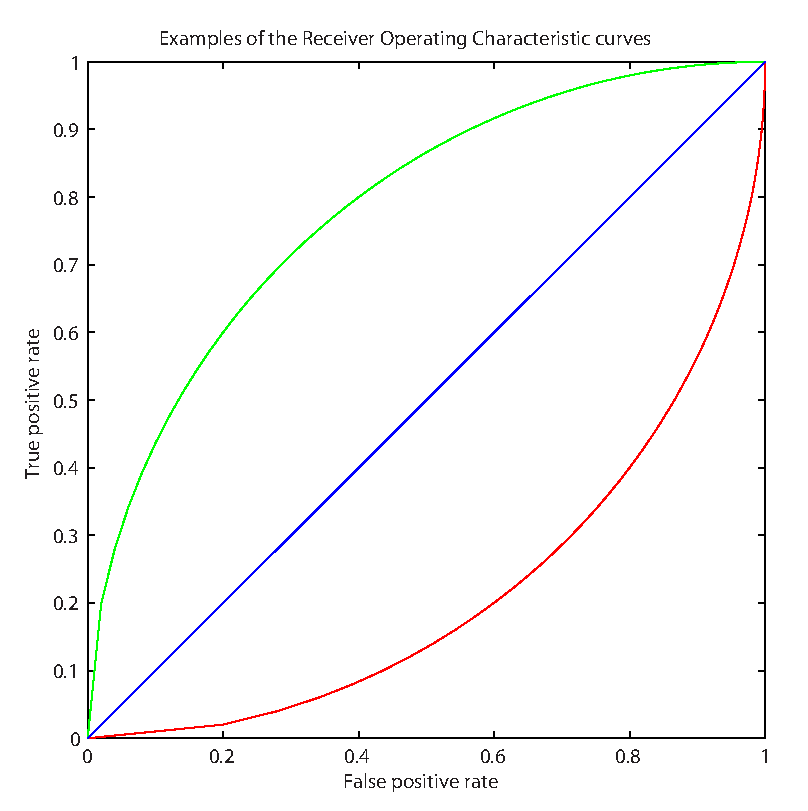
\includegraphics[width=0.55\columnwidth]{Figures/Chapter4/roc.pdf}
		\rule{37em}{0.5pt}
	\caption[Examples of the Receiver Operating Characteristic curves]{Examples of the Receiver Operating Characteristic curves}
	\label{fig:roc}
\end{figure}

\subsection{Speech/non-speech hit rates}

While the ROC curves capture the performance of a VAD algorithm across different thresholds, in practise, a single, fixed value is often chosen. This fact can have quite severe implications on algorithms whose best performance, captured by the ROC curve under many noise types and SNRs, exists at different thresholds. An algorithm cannot be called truly robust if it requires tweaking in its parameters to perform satisfactorily in various conditions. Therefore it is also important to evaluate the algorithms' performance with a single threshold value. Such evaluation can be carried out by plotting the so called \emph{speech hit-rate} (i.e. recall) and \emph{non-speech hit rate} (i.e. specificity) when the algorithms are implemented with a fixed threshold value, selected by examination of the ROC curves in different conditions. In this evaluation, the \emph{optimal} threshold has been identified by selecting the points on the ROC curves where the TPR and FPR are closest to being equal (in -5 and 0 dB SNRs) and calculating the mean of the corresponding threshold values while discarding the 2 most extreme ones.

%----------------------------------------------------------------------
%	SECTION 2 - Evaluation results
%----------------------------------------------------------------------

\section{Evaluation results}

In the two experiments, the selected VAD algorithms have been implemented and evaluated with and without the hang-over scheme described in Section \ref{sec:hang}. The ROC curves have been plotted for all six noise types at two low SNRs i.e. -5 dB and 0 dB. In order to capture the average performance, the AUC values have also been calculated. Finally, the most promising threshold for each algorithm across the two low SNRs and six noise types has been identified and the speech/non-speech hit rates at six different SNRs (20 dB to -5 dB) have been calculated.

In this chapter, only the results under two lowest SNRs (-5 dB and 0 dB) are going to be presented. Additional evaluation results for other SNRs have been put in Appendix \ref{AppendixA}.

\subsection{VAD algorithms with hang-over}

Figures \ref{fig:-5dBh} and \ref{fig:0dBh} present the ROC curves for all evaluated algorithms with hang-over for the six types of noise under -5 dB and 0 dB SNR respectively. In almost all cases, the LTSD algorithm (red line) seems to outperform all other VAD methods under both SNRs. In car noise, its performance is a bit worse than both the Sohn and Harmfreq's algorithms however it should be noticed that most algorithms perform exceptionally well in this type of noise. This can be explained by the fact that car noise occupies predominantly the low frequencies and the estimation procedure is able to track the noise well enough even at negative SNR. In factory noise, all algorithms seem to exhibit performance close to a random guess since all ROC curves are close to the 45$^\circ$ line.

The best average performance of the LTSD algorithm is confirmed by examination of the AUC values under -5 dB SNR presented in Table \ref{tab:AUC-5dBh} where the best value for the given noise type is highlighted in green while the worst one in red. The LTSD VAD outperforms all other algorithms in 4 out of 6 cases which results in the best average performance. On the other hand, the Entropy VAD is the worst performing algorithm in 5 out of 6 cases.

\begin{table}[htbp]
\center
\begin{tabular}{c|c|c|c|c|c|c!{\vrule width 1.5pt}c|}
\cline{2-8}
 & white & car & spchspect & babble & opsroom & factory & average \\ \hline
\multicolumn{1}{ |c| }{Sohn} & 0.8561 & 0.9595 & 0.9063 & 0.7786 & 0.8276 & 0.5671 & 0.8159\\ \hline
\multicolumn{1}{ |c| }{LTSD} & \textcolor{LimeGreen}{0.9497} & 0.9496 & \textcolor{LimeGreen}{0.9502} & \textcolor{LimeGreen}{0.8842} & \textcolor{LimeGreen}{0.8586} & 0.6345 & \textcolor{LimeGreen}{\textbf{0.8711}}\\ \hline
\multicolumn{1}{ |c| }{Entropy} & 0.9160 & \textcolor{red}{0.4999} & \textcolor{red}{0.5807} & \textcolor{red}{0.4832} & \textcolor{red}{0.4350} & \textcolor{red}{0.5315} & \textcolor{red}{\textbf{0.5744}}\\ \hline
\multicolumn{1}{ |c| }{PARADE} & \textcolor{red}{0.9117} & 0.8853 & 0.6159 & 0.5389 & 0.6339 & \textcolor{LimeGreen}{0.7071} & 0.7154\\ \hline
\multicolumn{1}{ |c| }{Harmfreq} & 0.9209 & \textcolor{LimeGreen}{0.9676} & 0.9126 & 0.7165 & 0.7992 & 0.6425 & 0.8265\\ \hline
\end{tabular}
\caption[AUC values of the evaluated algorithms \emph{with} hang-over under -5 dB SNR]{AUC values of the evaluated VAD algorithms \emph{with} hang-over under -5 dB SNR}
\label{tab:AUC-5dBh}
\end{table}

Finally, the speech/non-speech hit rates for the algorithms with hang-over and a fixed threshold are presented in Figure \ref{fig:snrh}. Again, the LTSD VAD exhibits the best speech detection characteristics, however remains slightly behind Harmfreq for the non-speech detection. It is worth reiterating that there is a trade-off between these two evaluation metrics and, especially for Harmfreq, lowering the threshold by a small value could increase the speech hit-rate while decreasing the non-speech's, bringing its performance close to the LTSD's.

\begin{figure}[htbp]
	\centering
		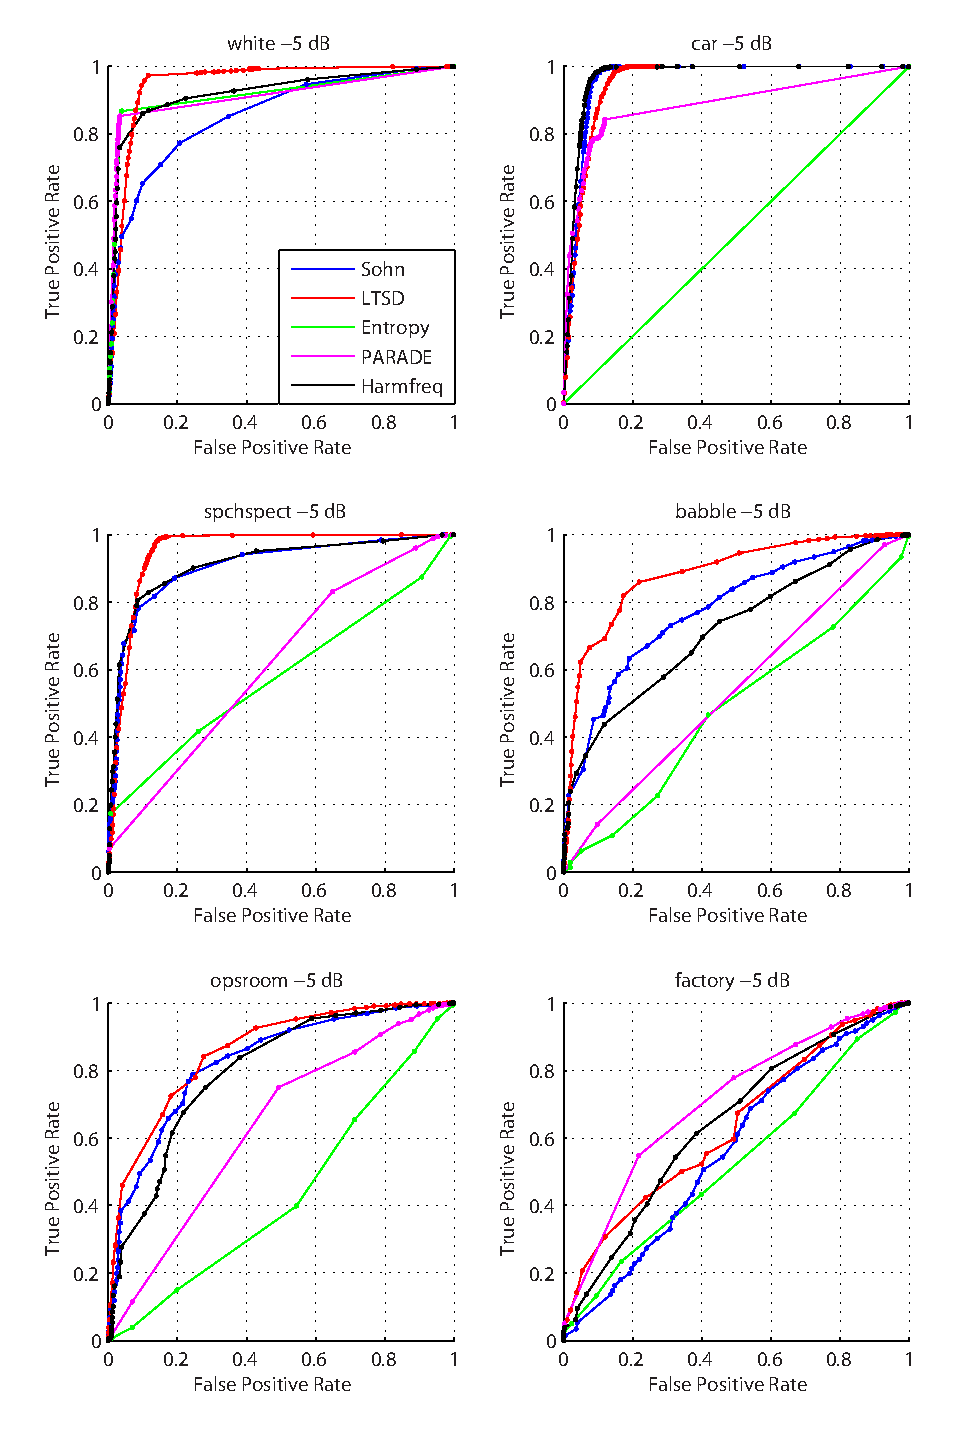
\includegraphics[width=1.0\columnwidth]{Figures/Chapter4/-5dBh.pdf}
		\rule{37em}{0.5pt}
	\caption[ROC curves of the evaluated algorithms \emph{with} hang-over under -5 dB SNR]{ROC curves of the evaluated VAD algorithms \emph{with} hang-over under -5 dB SNR}
	\label{fig:-5dBh}
\end{figure}

\begin{figure}[htbp]
	\centering
		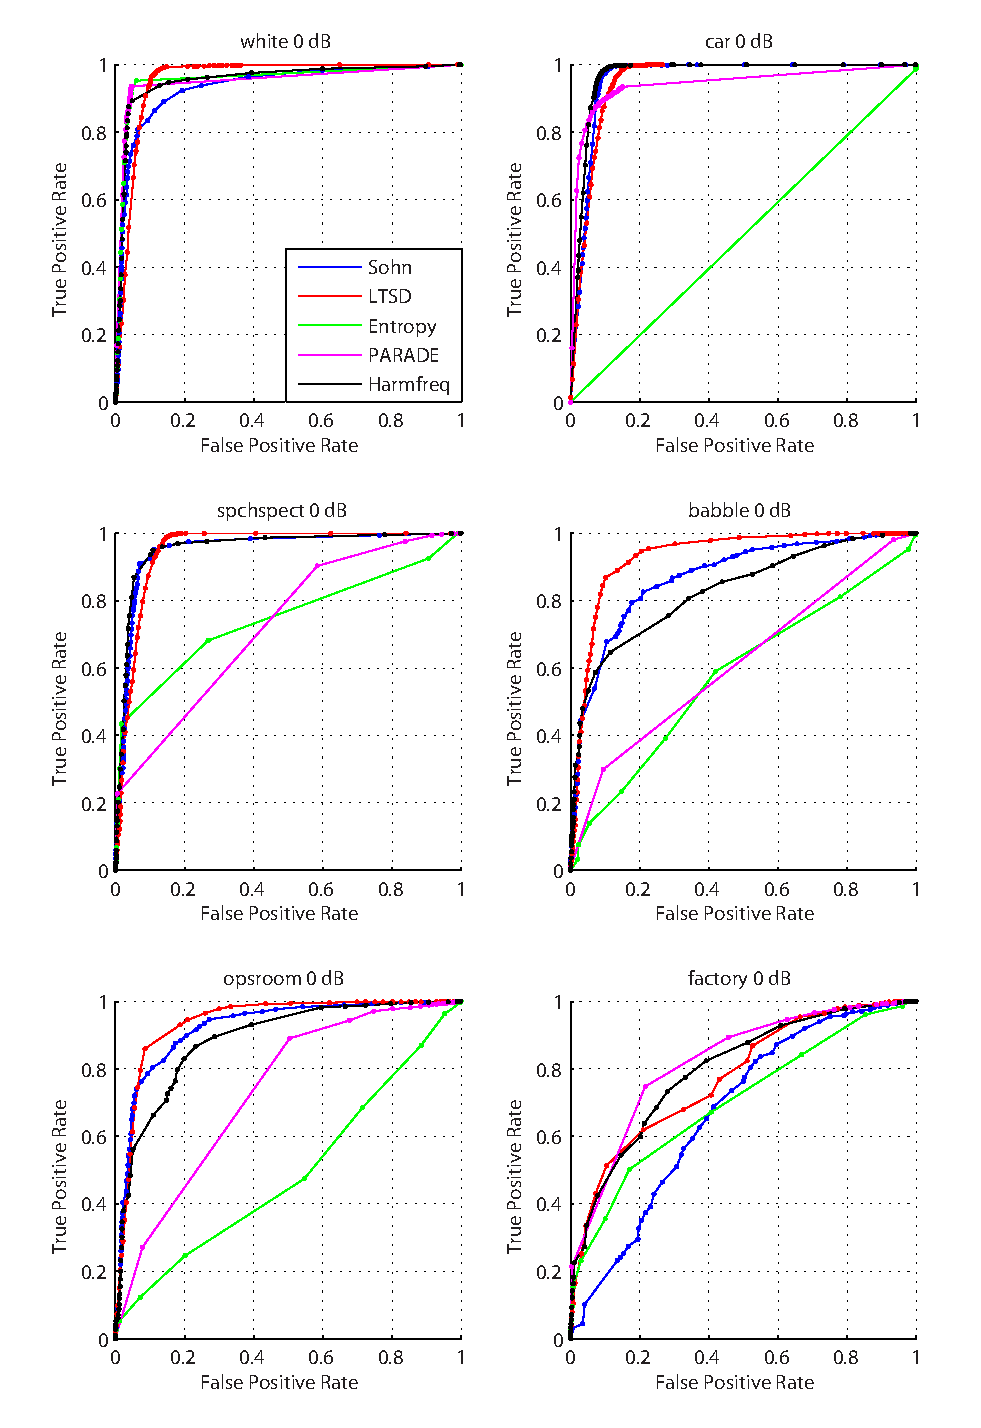
\includegraphics[width=1.0\columnwidth]{Figures/Chapter4/0dBh.pdf}
		\rule{37em}{0.5pt}
	\caption[ROC curves of the evaluated algorithms \emph{with} hang-over under 0 dB SNR]{ROC curves of the evaluated VAD algorithms \emph{with} hang-over under 0 dB SNR}
	\label{fig:0dBh}
\end{figure}

\begin{figure}[htbp]
	\centering
		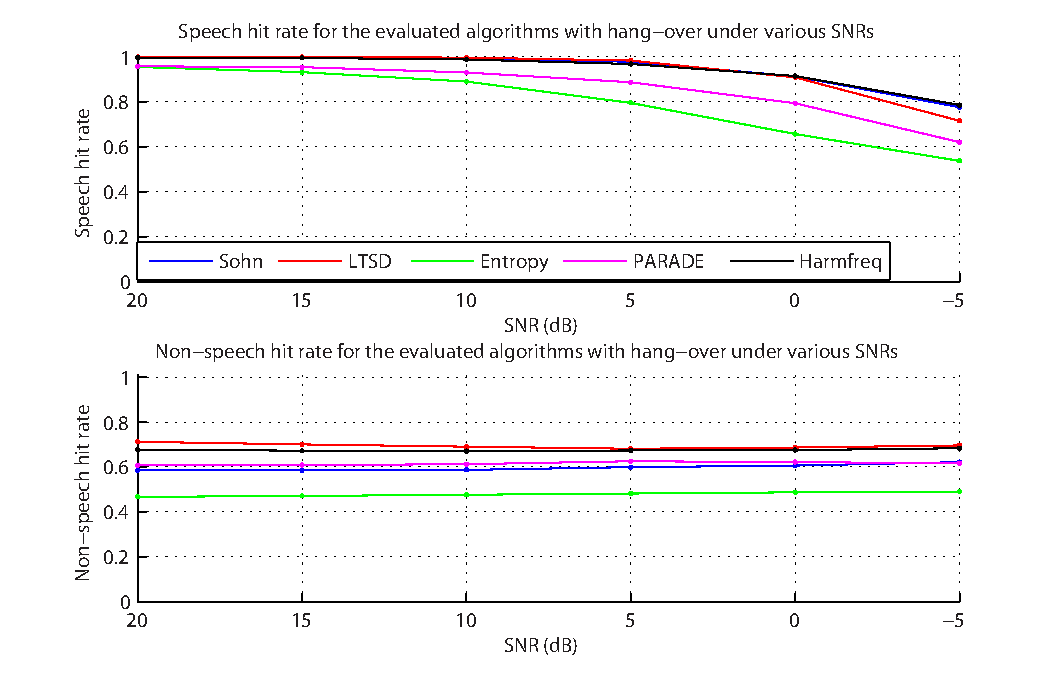
\includegraphics[width=0.9\columnwidth]{Figures/Chapter4/snrh.pdf}
		\rule{37em}{0.5pt}
	\caption[Speech/non-speech hit rates for the evaluated algorithms \emph{with} hang-over under different SNRs]{Speech/non-speech hit rates for the evaluated algorithms \emph{with} hang-over under different SNRs}
	\label{fig:snrh}
\end{figure}

\subsection{VAD algorithms without hang-over}

The same algorithms have also been implemented without the hang-over scheme. It can be argued that this is a more objective evaluation of the VAD features since the algorithms stop immediately after the thresholding stage. However, the harmonicity based algorithms are likely to underperform if implemented without the hang-over scheme. Similarly to the previous section, Figures \ref{fig:-5dBnoh} and \ref{fig:0dBnoh} present the ROC curves under -5 dB and 0 dB SNR. Again, the LTSD VAD performs best, while the Entropy VAD exhibits the worst performance. Interestingly, the LTSD's results indicate that the version without hang-over operates better in car noise than the one with. This can be explained by an observation that LTSD without hang-over already achieves such a good performance that when combined with a smoothing scheme, it stretches the speech labels beyond the actual utterances which results in an additional number of false positives.

The best average performance of the LTSD VAD is again confirmed by the AUC values presented in Table \ref{tab:AUC-5dBnoh}. By comparing the two AUC tables (i.e. with and without hang-over) it can be noticed that the LTSD algorithm benefits least from the hang-over scheme. On the other hand, Harmfreq's performance is boosted to the greatest extent. Examination of the speech/non-speech hit rates with a fixed threshold in Figure \ref{fig:snrnoh} again confirms that the LTSD algorithm exhibits the best performance, this time both in the speech as well as in non-speech hit rates.

\begin{figure}[htbp]
	\centering
		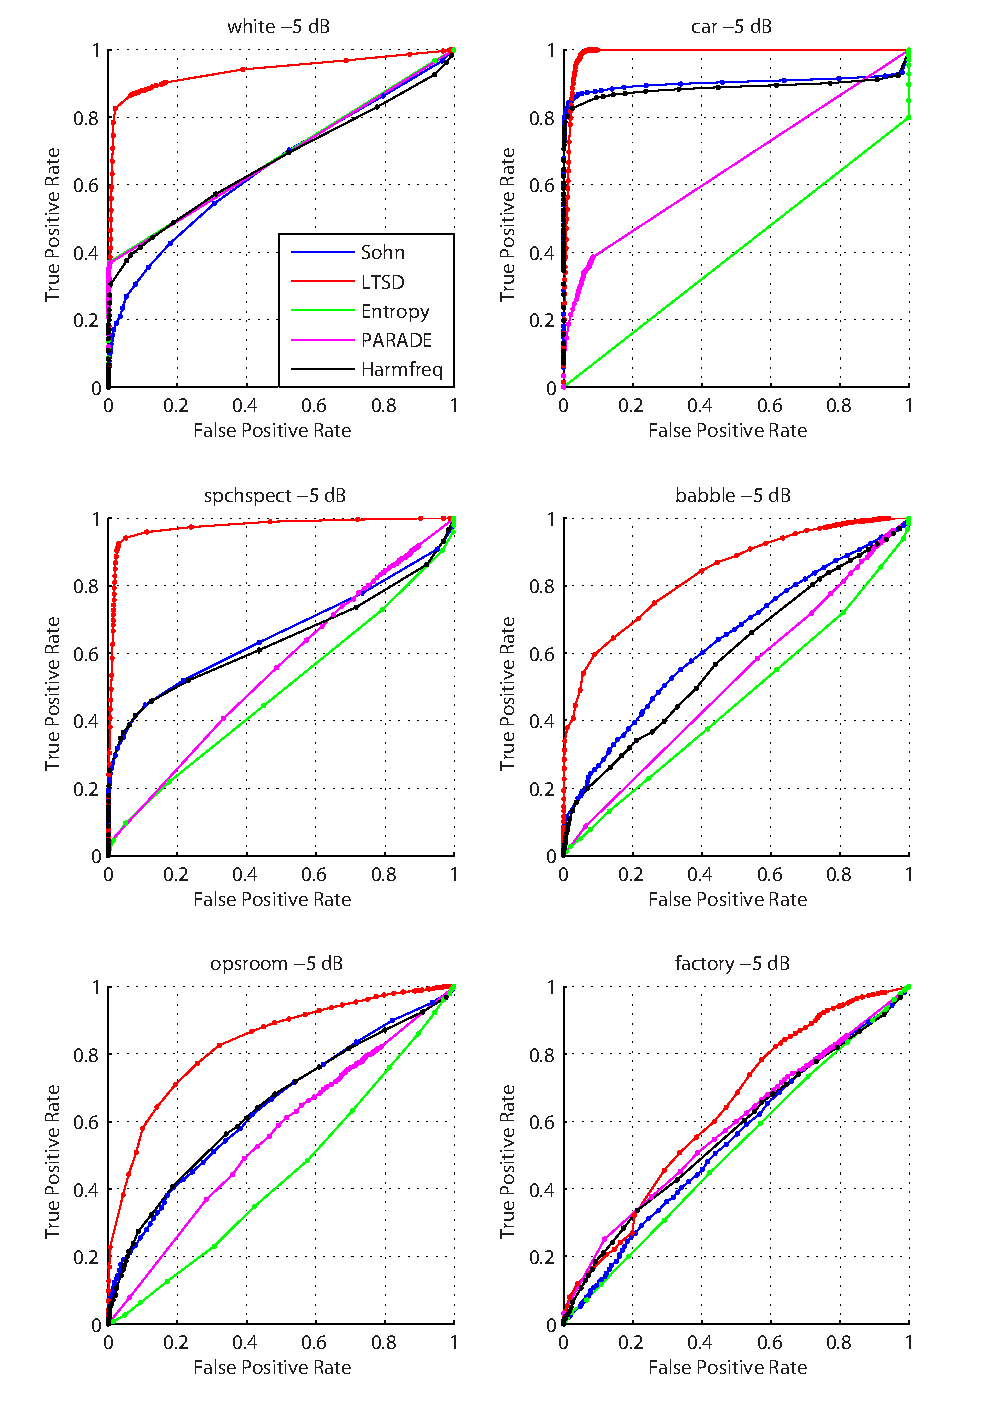
\includegraphics[width=1.0\columnwidth]{Figures/Chapter4/-5dBnoh.pdf}
		\rule{37em}{0.5pt}
	\caption[ROC curves of the evaluated algorithms \emph{without} hang-over under -5 dB SNR]{ROC curves of the evaluated VAD algorithms \emph{without} hang-over under -5 dB SNR}
	\label{fig:-5dBnoh}
\end{figure}

\begin{table}[htbp]
\center
\begin{tabular}{c|c|c|c|c|c|c!{\vrule width 1.5pt}c|}
\cline{2-8}
 & white & car & spchspect & babble & opsroom & factory & average \\ \hline
\multicolumn{1}{ |c| }{Sohn} & 0.6540 & 0.9019 & 0.6564 & 0.6378 & 0.6423 & 0.5424 & 0.6725\\ \hline
\multicolumn{1}{ |c| }{LTSD} & \textcolor{LimeGreen}{0.9365} & 0.9876 & \textcolor{LimeGreen}{0.9741} & \textcolor{LimeGreen}{0.8362} & \textcolor{LimeGreen}{0.8323} & 0.6339 & \textcolor{LimeGreen}{\textbf{0.8668}}\\ \hline
\multicolumn{1}{ |c| }{Entropy} & 0.6856 & \textcolor{red}{0.4007} & \textcolor{red}{0.4878} & \textcolor{red}{0.4561} & \textcolor{red}{0.4425} & \textcolor{red}{0.5160} & \textcolor{red}{\textbf{0.4981}}\\ \hline
\multicolumn{1}{ |c| }{PARADE} & \textcolor{red}{0.6821} & 0.6563 & 0.5514 & 0.5156 & 0.5542 & \textcolor{LimeGreen}{0.5810} & 0.5901\\ \hline
\multicolumn{1}{ |c| }{Harmfreq} & 0.6696 & \textcolor{LimeGreen}{0.8873} & 0.6392 & 0.5912 & 0.6433 & 0.5648 & 0.6659\\ \hline
\end{tabular}
\caption[AUC values of the evaluated algorithms \emph{without} hang-over under -5 dB SNR]{AUC values of the evaluated VAD algorithms \emph{without} hang-over under -5 dB SNR}
\label{tab:AUC-5dBnoh}
\end{table}

\begin{figure}[htbp]
	\centering
		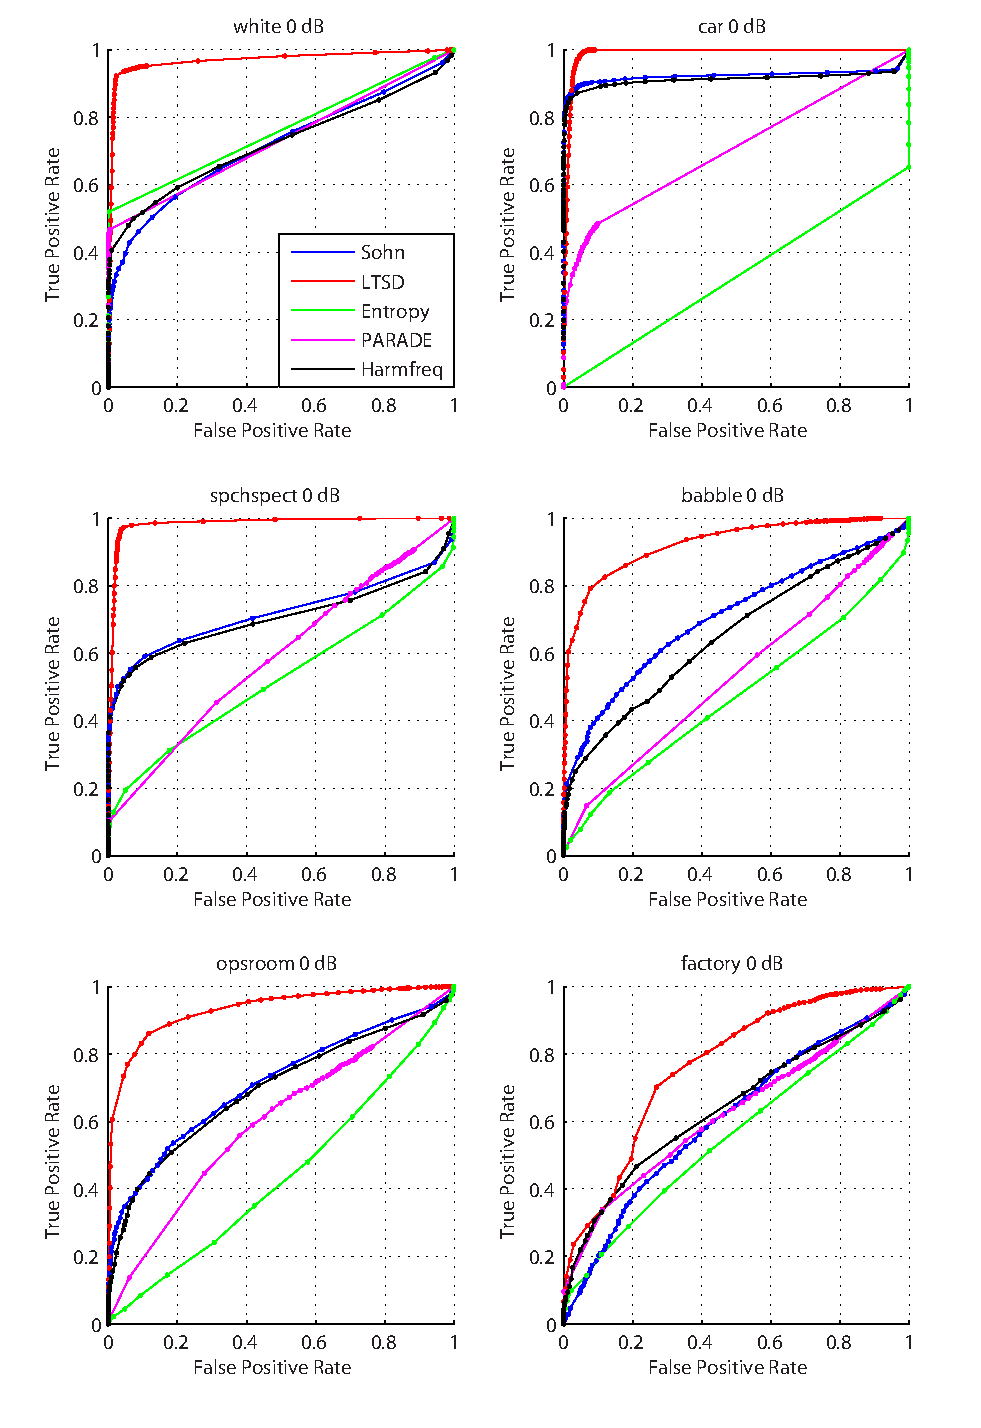
\includegraphics[width=1.0\columnwidth]{Figures/Chapter4/0dBnoh.pdf}
		\rule{37em}{0.5pt}
	\caption[ROC curves of the evaluated algorithms \emph{without} hang-over under 0 dB SNR]{ROC curves of the evaluated VAD algorithms \emph{without} hang-over under 0 dB SNR}
	\label{fig:0dBnoh}
\end{figure}

\begin{figure}[htbp]
	\centering
		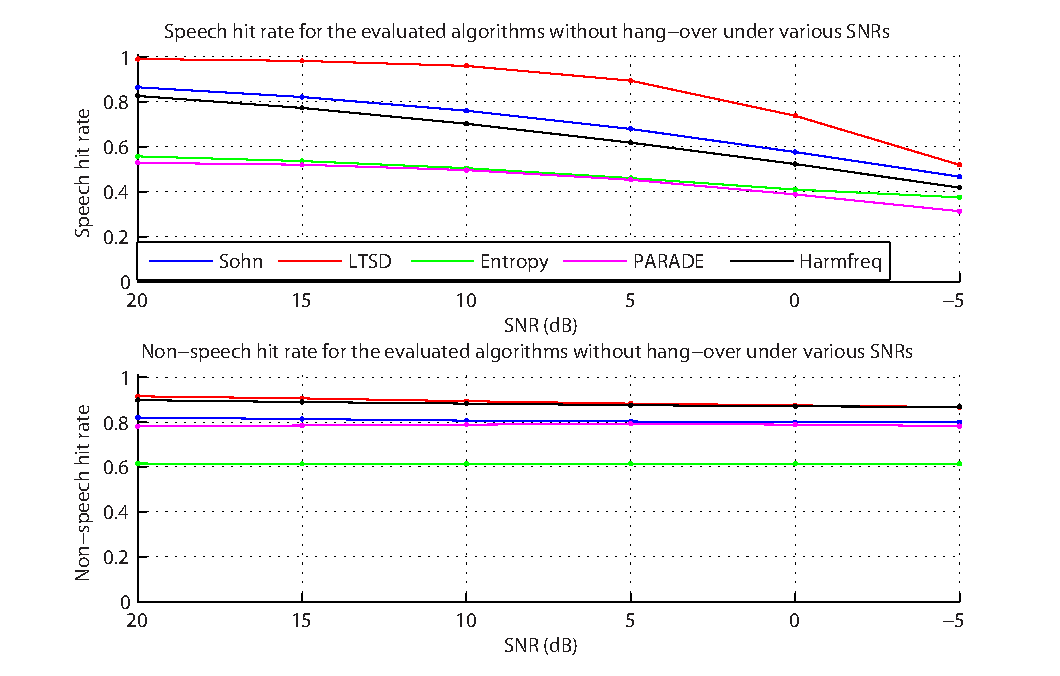
\includegraphics[width=0.9\columnwidth]{Figures/Chapter4/snrnoh.pdf}
		\rule{37em}{0.5pt}
	\caption[Speech/non-speech hit rates for the evaluated algorithms \emph{without} hang-over under different SNRs]{Speech/non-speech hit rates for the evaluated algorithms \emph{without} hang-over under different SNRs}
	\label{fig:snrnoh}
\end{figure}

%----------------------------------------------------------------------
%	SECTION 2 - Conclusion
%----------------------------------------------------------------------

\section{Conclusion}

The evaluation results confirm the hypothesis that the best algorithm cannot be identified for all conditions, which in the real world there are infinitely many of. However, for the evaluated noise types, the LTSD algorithm exhibits the best average performance in 4 out of 6 cases, as concluded from the analysis of Tables \ref{tab:AUC-5dBh} and \ref{tab:AUC-5dBnoh}. Therefore, for practical use, it is beneficial to narrow down the conditions in which the algorithm will have to operate as much as possible. Then, all algorithms can be properly benchmarked and the best one for the specific application could be chosen. Should this be impossible, the best bet is probably to use the LTSD VAD, at least from all the algorithms evaluated in this work.